%!TEX root = ../main.tex

%%%%%%%%%%%%%%%%%%%%%%%%%%%%%%%
%%%%%%%%%%%%%%%%%%%%%%%%%%%%%%%
\chapter{Methodical Modeling}
\label{chap:methodical-modeling}

\begin{textblock*}{.7\textwidth}(70mm-\offset,25mm-\offset)
        \begin{fquote}[Albert Einstein]
            All models are wrong, but some are useful.
        \end{fquote}
\end{textblock*}

This chapter mehodical modeling focusses on the description of thoughs and structures of the implementation in Python.
It is not evolving more than necessary details about the package {\itshape diffpssi}, but trying to comprehensible illustrate the structure of the algorithms theirselves and the necessaary bordering interfaces.

%%%%%%%%%%%%%%%%%%%%%%%%%%%%%%%
%%%%%%%%%%%%%%%%%%%%%%%%%%%%%%%
\section{Transformer Equipment Modeling}
\label{sec:transformer-modeling}

This section respectively focusses on the dynamics and model behavior of the transformer itself.
It is split according to the structure of the implementation itself, into the modeling of the $\Pi$-model and the tap changer control.
For the last mentioned, there are different control schemes implemented and thus described in the subsequent section.
In the beginning, the rough software structure idea of the extension is described, continuing with a dive into the mathematical relations, and specialities.  

%%%%%%%%%%%%%%%%%%%%%%%%%%%%%%%
\subsection{Software Architecture Design}
\label{sec:modeling-architecture}

The first scope of the \textit{diffpssi} extension is to form a modular and easy to maintain class structure. 
The background is to enable support of adding other types of transformers and resp. or connected control circuits.
A conceptual chart of this architecture is shown in \autoref{fig:transformer-architecture}.
It is representing only necessary classes or packages for the transformer and its control.

\begin{figure}[htbp!]
        \centering
        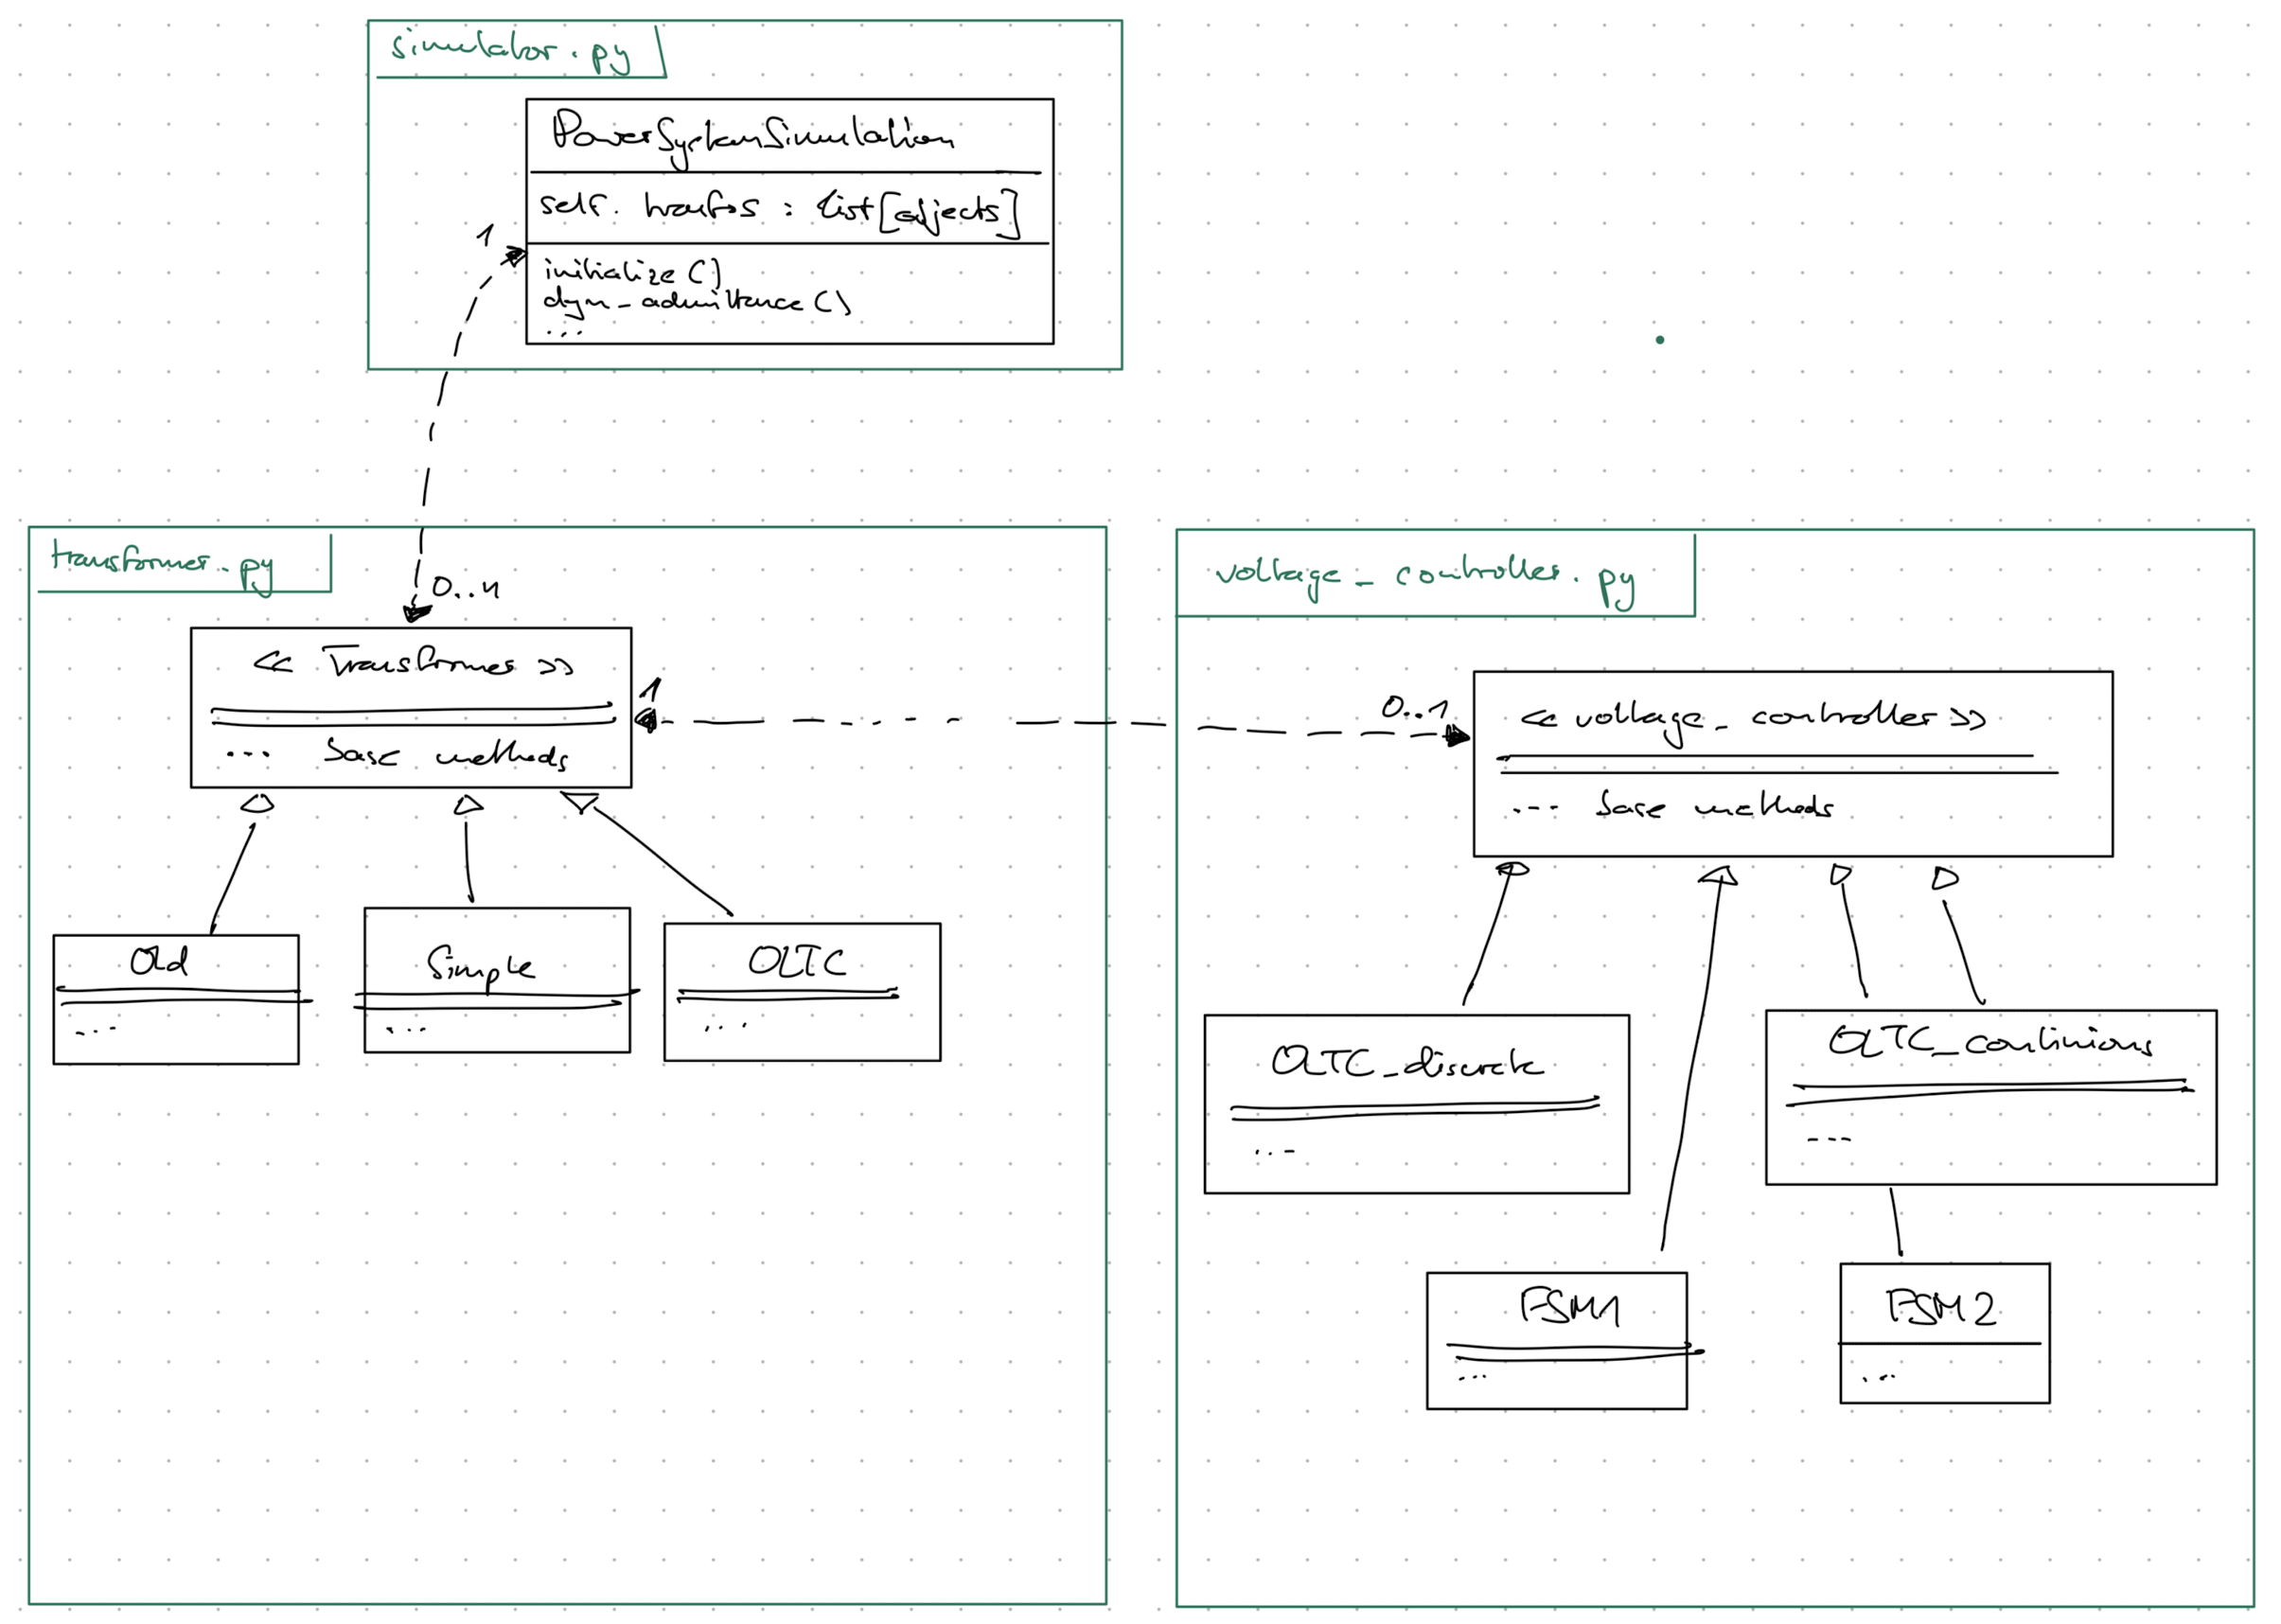
\includegraphics[angle=90, width=\linewidth]{modeling/diffpssi_trafo_architecture.png}
        \caption[Architecture of the implemented models in \textit{diffpssi}]{Architecture of the implemented models in \textit{diffpssi}; Using abstract classes for correct interfaces and improved reusability; only necessary packages, modules and classes are depicted}
        \label{fig:transformer-architecture}
\end{figure}

%%%%%%%%%%%%%%%%%%%%%%%%%%%%%%%
\subsection{Implementing a $\Pi$-Representative Circuit with Variable Ratio}

Before detailing in the software side of the implemetation, some mathematical differences are explained.
This results on the one hand from the major differences in the standard literature, especially between \textcite{machowski_2020} and \textcite{kundur_2022}, resp. \textcite{milano_2010}.
On the other hand, these differences occur as well in the comparative and validation simulation software \textit{DIgSILENT PowerFactory}.
The use of these different models is described in its technical reference manual \quelle. 

%%%%%%%%%%%%%%%%%%%%%%%%%%%%%%%
\subsubsection{Mathematical Description and Definitions}

\sidenote{Important definitions and literature differences}
Firstly it is important to comment on the use of indices in this thesis, and especially following for this chapter.
The index 1 is always referring to the \acs{LV} side, the index 2 to the \acs{HV} side. 
The impedances can be concentrated and related to either the \acs{LV}, or as usual to the \acs{HV} side of the transformer. 
The in \autoref{sec:trafo-model} used derivation is using a relation on the \acs{HV} side.
The same accounts for the definition of the \acs{OLTC} ratio $\underline{\vartheta}$.     
The \acs{OLTC} ratio $\underline{\vartheta}$ in this thesis is always placed on the HV side.
% If one wants to place this ratio on the \acs{LV} side, the in this thesis defined ratio has to be used reciprocal.
% For the simulation tool, this is crucial to understand and define correctly in order to acquire correct results.

\sidenote{Definition OLTC ratio}
This thesis focusses on an ideal tap changer model at first, other possible considerations from \autoref{sec:further-considerations} are neglected.
As vector groups are as well not considered, the tap ratio stays solely a rational number.
Like previously mentioned, and consequently described, the ratio $\vartheta$ is then pülaced on the \acs{HV} side of the transformer.
The \acs{OLTC} ratio $\vartheta$ is then defined as:
\begin{align}
        \vartheta_\mathrm{HV} &= 1 + k \cdot \Delta v \label{eq:tap-ratio-hv} \\[6pt]
        \text{with } k &\in [k_\mathrm{min};k_\mathrm{max}]; k_\mathrm{min} \equiv  -k_\mathrm{max} \label{eq:tap-pos}
\end{align}
Within this definition, $k_\mathrm{min}$ defines the minimum tap position, $k_\mathrm{max}$ the maximum \acs{OLTC} position. 
The variable $\Delta v$ defines the change of the ratio in percent for alterning one position.

% \sidenote{Representation of\\Vector Groups}
% Voltage angle shifting through the influence of vector groups, meaning a different wiring and thus magnetic coupling of the transformer can be expressed within the transformer model. 
% By mathematically applying a turning vector with the length of one to the overall tap ratio, this can be included in the model. 
% Mathematical, this is expressed by the following equation. 
% The characteristic number $n_\mathrm{T}$ is relating to to angle, with one step being equal to $30^\circ$ angle ratio.
% \begin{align}
%         \underline{a}_\mathrm{T} &= \exp(j \cdot n_\mathrm{T} \cdot \frac{\pi}{6}) \label{eq:vector-group}
% \end{align}

\subsubsection{Mathematical Different Representations}
\sidenote{Relation to the LV side}
When one either wants to relate the transformer admittance, or the tap ratio to the \acs{LV} side, a different admittance matrix definition has to be used.
The admittance matrix is then defined as:
\begin{align}
        \underline{\mab{Y}}_\mathrm{\Pi,T}&= 
        \begin{bmatrix}
            \underline{Y}_\mathrm{T} & -\underline{\vartheta}\underline{Y}_\mathrm{T} \\
            \underline{\vartheta}^*\underline{Y}_\mathrm{T} & -\underline{\vartheta}^*\underline{\vartheta}\underline{Y}_\mathrm{T}
        \end{bmatrix} \label{eq:admittance-oltc}
    \end{align}
The following mathematical result leads to a necessary change in the software implementation.
Either \mycomment[MK]{Is this actually the case? Or is it a different condition?}
\begin{itemize}
        \item the admittance matrix bus indices have to be changed,
        \item the tap ratio has to be reciprocal according to \autoref{eq:tap-ratio-lv}, or
        \item using the \acs{HV} side admittance matrix, but changing the tap ratio definition and the bus indices.
\end{itemize}
These different ways of variable and placing definitions also characterize the ways, the admittance matrix of the \acs{OLTC} transformer is derived from either \textcite{machowski_2020}, versus \textcite{kundur_2022}, \textcite{milano_2010}, or \textcite{burlakin_2024}.
Another thought or way of representing a transformer with off-nominal ratio is described in the appended \autoref{app:current-injection-model}.
\begin{align}
        \vartheta_\mathrm{LV} &= \frac{1}{1 + k \cdot \Delta v} \label{eq:tap-ratio-lv}
\end{align}

\subsubsection{Thoughts, Design, and Implemetation of Algorithmics}

\commenting{
        Base idea here: 
        \begin{itemize}[nosep]
                \item Show the thought process, design sketches and the implemetation algorithmics in the Python framework.
                \item Add a class diagram of the transformer model, with all needed interface / logable data, interface methods, and the abstract design.
                \item Describe addtional methods.
                \item Show the algorithmic implemetation logic of the Pi model, but not the Tap Changer, as this is seperated. 
        \end{itemize}
        Additionally interesting extensions:
        \begin{itemize}[nosep]
                \item How to automatically determine switching direction?\\
                -> switchin direction dependent on what? (load-flow direction?)
                \item Controller set points: also dependent on load flow?
                \item How can I change the transformer control setpoints to be load flow dependent?
                \item How can I ensure, utilization of the transformer is not $>S_\mathrm{n}$?
        \end{itemize}
}

%%%%%%%%%%%%%%%%%%%%%%%%%%%%%%%
\subsection{Tap Changer Control Modeling}
\label{sec:modeling-tap-changer-control}

\commenting{This is the description of the ideas, development, and implementation of a OLTC control scheme.}


\subsubsection{Discrete Control Loop}
\commenting{
        \begin{itemize}[nosep]
                \item Describe implementation
                \item Describe benefits / drawbacks
                \item Control scheme
                \item Switching logic and behavior (voltage tracking)
        \end{itemize}
}

\sidenote{General aspects\\and references}
This control method represents the currently most used and thus representative control scheme for \acsp{OLTC}. 
With the mechanic nature of the switching mechanism, the control look can only access discrete ratios within time frames of around a few seconds. 
Such a discrete control loop is described by \textcite{milano_2011,milano_2010}. 
A scheme of this control loop is shown in \autoref{fig:discrete-control-loop}.

\begin{figure}[htb!]
        \centering
        \missingfigure{Discrete control loop}
        \caption{Discrete control loop of an \acs{OLTC}; scheme based on \textcite{milano_2011}}
        \label{fig:discrete-control-loop}
\end{figure}

This control loop type is beneficial due to its accurate representability of current \acs{OLTC} abilities. 
It gains access to assess stability within simulation environments, as analytical methods are not suited.

A negative aspect of a discrete control loop is the missing opportunity of generating a transfer function. 
This blocks the stability assessment with standard control engineering methods. 
Further, popular analysis methods like eigenvalue analysis is not possible, due to the lack of possibility to form derivatives.

% \lstinputlisting[caption={Output Function of the discrete OLTC controller},captionpos=b,style=style-python,label=lst:oltc-discrete]{images/code/oltc-discrete.py}

\sidenote{Implementation\\Structure}
\commenting{The structure of the implementation is illustrated in the block diagram of \autoref{fig:discrete-oltc-implementation}. 
The controller is actively chainging the algebraic funtions of the simulation environment, therefore it is quasi dynamic. 
The controller output logic is called, when updating the admittance matrix of the transformer. 
Additionally, the differential functions of the connected simple controllers, like integrators, PT1-blocks, etc., are called by the solver and are thus part of the differential equations. 
The logic determines the physical interpretation of the \acs{OLTC}, and therefore
\begin{enumerate}
        \item If the OLTC has to switch,
        \item When the switching operation is finished, and
        \item What the current, or in case after a switching the new, tap ratio is.
\end{enumerate}
It is important to note, that this structure relies on the calculation of the dynamic admittance matrix on each time step.}

\begin{figure}[htb!]
        \centering
        \missingfigure{Implementation structure of the discrete OLTC controller}
        \caption[Implementation structure of the discrete OLTC controller]{Implementation structure of the discrete OLTC controller}
        \label{fig:discrete-oltc-implementation}
\end{figure}

\sidenote{Output logic}
The output of the controller is based on the following logic.

\sidenote{Characterization plot and validation}

% \lstinputlisting[caption={Output Function of the discrete OLTC controller 2},captionpos=b,style=style-python,label=lst:oltc-discrete2]{images/code/oltc-discrete.py}

\subsubsection{Continous Control Loop}

\begin{figure}[htb!]
        \centering
        \includegraphics[width=.7\linewidth]{development_files/validation/data/oltc_control_characterization.pdf}
        \caption[Characterization of the OLTC control loops]{Characterization of the OLTC control loop; the input function simulates the to be regulated voltage, the output functions are characterized by $o(t)=i(t) \cdot \underline{\vartheta}_\mathrm{trafo}$}
        \label{fig:oltc-control-characterization}
\end{figure}

\subsubsection{Control Schemes for the Fast Switching module}

\commenting{\textbf{ATTENTION:} Two models availabel, described in the paper, where the FSM is preferred and the 'novel' scheme where usage of FSM or OLTC ios dependent on the tap skipping and the deas band. Only the last is usable for verification!}

\commenting{
        \begin{itemize}[nosep]
                \item Describe implementation
                \item Describe benefits / drawbacks
                \item Control scheme
                \item Switching logic and behavior (voltage tracking)
        \end{itemize}
}
\sidenote{Functional basics\\of a \acs{FSM}}
Describe the operational logic and structure of the \acf{FSM} first.

\sidenote{Control logic}
A control logic for a so called \acs{FSM} has been presented from \textcite{burlakin_2024}, and illustrated in \autoref{fig:fsm-control-loop}.

\begin{figure}[htb!]
        \centering
        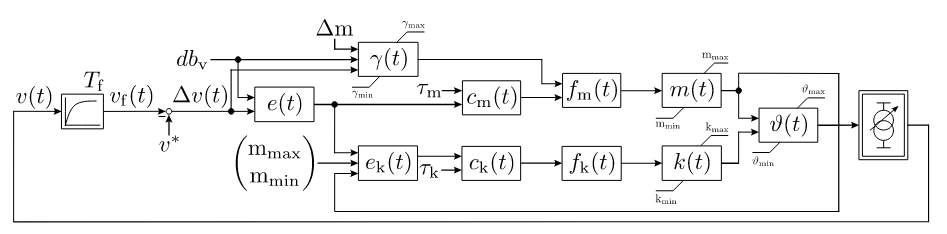
\includegraphics[width=\textwidth]{modeling/fsm_control_scheme.png}
        \caption[Control loop of a \acf{FSM}]{Control loop of a \acs{FSM}; scheme based on \textcite{burlakin_2024}}
        \label{fig:fsm-control-loop}
\end{figure}

\sidenote{Implementation\\differences}
However, the implementation logic in Python is slightly differing from the presented scheme in \autocite{burlakin_2024}, simply for not overcomplication of the code and therefeore debugging. 
The implementation is similar to the afore discussed one of a standard \acs{OLTC} controller. 

\sidenote{Characterization\\and validation}

%%%%%%%%%%%%%%%%%%%%%%%%%%%%%%%
\subsection{Experimental: Extended Ideas and Improvements}

\subsubsection{Operational Oriented FSM Control}

\ai{
        The time constants are used in the control model to model the influnce of switching operation duration.
        This is coming from the mechanical movement of the OLTC, therefore it is the \glqq maximum possible dynamic behavior\grqq.
        The FSM doesnt't have this limitation, as it can switch after every $\sin$ period (0.02 s).
        
        Currently we can access two different operational modes: Prefer the FSM, or switching on how far is the voltage deviated in both time constants.
        This is a first, more targeted approach towards concerning dynamics in the voltage behavior, but still based on the time constants, not only limited through them.
        
        Why don't we approach a control strategy, which is only considering dynamics, and let the time constants just restrain and block the switching.
        Meaning, that the faster the voltage deviates, the more the FSM gets preferred, the slower the dynamics, the more the standard OLTC gets preferred.
        This could also lead to neglecting a dead-band, and still preventing so called tap-hunting.

        Combined with an operational oriented thought, keeping the possible switching movements of the FSM at its maximum / optimal position.
        This would mean, that in more static times, the FSM switches in its defined \glqq as neutral defined\grqq position and the OLTC is balancing the devaitions.
        One might call this a corrective supervision or monitoring.
}

\subsubsection{Alternative Tap Skipping Logic}

\ai{
        Curretnly the tap skipping logic is formulated as
        \begin{quote} \itshape
                How many times does the deadband fit into the voltage deviation?
        \end{quote}
        to determine the floored number of skips (with contraints). 
        Meaning in mathematical terms: 
        \begin{align}
                \eta(t)=\text{floor}\bigg(\frac{\vert \Delta v(t)\vert}{db_\mathrm{v} \cdot \Delta m}\bigg)
        \end{align}

        An alternative approach would be: 
        \begin{quote} \itshape
                How many switches of the FSM would the current offset voltage bring back to the reference value?
                How many times does one FSM switch fit into the voltage deviation?
        \end{quote}
        Meaning in mathematical terms:
        \begin{align}
                \eta(t)=\text{floor}\bigg(\frac{\vert \Delta v(t)\vert}{\Delta k \cdot \Delta m}\bigg)
        \end{align}
        
        Last approach should be more accurate for different pairs of preset values (deadband, added voltage per tap, etc.).
        BUT: both approaches do not consider the true effect on the dynamic loads and the grid.
        Different grid strengths could react differently on the applied transformer ratio.
}

\subsubsection{Varying the Voltage Setpoint and Target Calculation}

\commenting{
        Here, another idea of control target creation shall be mentioned. 
        Instead of a fixed bus voltage reference, the difference of both bus voltages is considered. 
        Further, the sign of that difference is used to determine the direction of the tap change.
}

\ai{
        Different things to consider here:
        \begin{itemize}
                \item \textbf{Load-flow Direction} with ranking the bus voltages in p.u. against each other,
                \item \textbf{Dynamic Setpoints} through automated calculation of target voltage (nose curves),
                \item \textbf{Different Control Input} as not with a fixed target value, but the difference between both bus voltages; thus tentiative, becuase it is not considering supporting the load, but falsly trying to prevent a wrong switching direction.
        \end{itemize}
}


%%%%%%%%%%%%%%%%%%%%%%%%%%%%%%%
%%%%%%%%%%%%%%%%%%%%%%%%%%%%%%%
\section{Application of Voltage Stability}
\label{sec:application-voltage-stability}

% Combined with the nose curves, critical points shall be identified, highlighted, and characterized.
% Additionally to help this highlighting and characterization, one index based of the nose curves for linearization of remaining distance to the critical point is added. 

As previously discussed in the fundamentals of voltage stability, \autoref{sec:voltage-stability}, ensuring power quality is a secondary goal.
Concerning that voltage stability, regardless of short- or long-time evaluation, is a topic of power quality, it is hard to determine stability or instability.
In terms of static possible solutions, there are a lot of tools determing the critical points, as well as the current distance to it.
Looking into the short-term, more dynamic assessment, there are less elegant solutions. 
This thesis is trying to keep the perspective on both, short- and long term voltage stability.
The following is the approach to synthesize a toolset for voltage stability analysis, that is at least dynamically comparable.
As nose curves are a valid and popular tool, they shall be implemented first. 
Afterwards the time series calculation is tried to integrate into this static evaluation, including tap changer dependent behavior.
Lastly, a more dynamic rating of a sceario shall be computed, enabling also the confirmity with grid codes for example.

%%%%%%%%%%%%%%%%%%%%%%%%%%%%%%%
\subsection{Generation of Nose Curves}
\label{sec:nose-curves}

\commenting{NOTE: Please reconsider and remake this section after completation of the Rating Tool / Assessment Method.}

This section describes the implementation of a prevoiusly discussed static voltage analysis tool.
The generation of nose curves helps in finding the critical loading of the system at the bus of interest, although it is static nature. 

\subsubsection{Basic Simplification Idea}

\textcite{ajjarapu_1992, ajjarapu_2007} are presenting a method for numerical calculation of nose curves in their work. 
It is called {\itshape Continuation Power Flow} and is based on a modified Newton-Raphson method.
The differences rely in a slightly different definition of the power flow equations, considering a load factor $\lambda$.
Combined with a predictor-corrector iterative solver method, this algorithm is capable of nose curve calulation, and finding the critical loading of the system.
While in the first work \autocite{ajjarapu_1992}, only the upper part of the curve including the critical point is calculated, the second work \autocite{ajjarapu_2007} is capable of calculating the complete curve with both solutions. 
As the trade off between implementation effort and the benefits, this method is not exchanging the reduced and simplyfied one.

While this method would be appealing to implement, an additional load flow algorithm, solver, and wrapper seem not profitable for this thesis.
An idea was occuring, just iteratively using the available implemented standard Newton-Raphson algorithm, and implementing a wrapper around it.
The proposed result should be the upper and stable nose curve branch, with the critical point of active power loading.
This shall seem sufficient, as the lower branch solutions are not stable load flow solutions.

The often used parameterization of a function of voltage dependent on the active power and the power angle $\phi$ should be implemented.
In mathematical term, this is expressed as \autoref{eq:pv-mathematical}.
\begin{align}
        \vert \underline{V} \vert : P &\mapsto f(P, \phi) \label{eq:pv-mathematical} \\[6pt]
        Q : \underline{V} &\mapsto f(\underline{V}, \phi) \label{eq:vq-mathematical}
\end{align}
Under consideration of a complex representation of voltage and powers, this algorithm can calculate $V-Q$ curves as well. 
Mathematically this is expressable as \autoref{eq:vq-mathematical}.

\subsubsection{Implementation Details}

\begin{wrapfigure}[12]{r}{0.4\textwidth}
        % \vspace{-20pt}
        \centering
        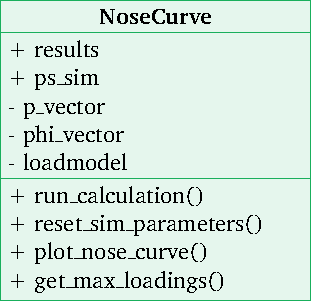
\includegraphics[width=.9\linewidth]{tikz_graphics/images/class_diagram_nosecurve_red.pdf}
        \caption{Class diagram of the NoseCurve class in the package diffpssi}
        \label{fig:nose-curve-characterization}
\end{wrapfigure}
The implementation of the nose curve generation is realized as a class in the package {\itshape diffpssi.stability$\_$lib.voltage}.
Its class diagram with all attributes and methods is shown in \autoref{fig:nose-curve-characterization}, an extended version is included in \autoref{app:nose-curve}.
For an easy and generic use of the {\itshape diffpssi} package, {\itshape PowerSystemSimulation} objects are used, as well as the function {\itshape do$\_$load$\_$flow()} from the package.

As the afore mentioned idea, the method for running the calculation is a iterative wrapper of the load flow calculation. 
This can be as well applied for mutiple busses as a list input.
At first, the grid and therefore models of the {\itshape PowerSystemSimulation} object has to be cleared with the method {\itshape reset$\_$sim$\_$parameters()}.
Then the active power vector is iterated as load input, together with the power angle $\phi$ for the reactive power in the model.
Important to note here, is the usage of an {\itshape **kwargs} argument.
The callable for the model is called with load parameters for each load bus as the Bus name, and a list with active and reactive power.
The initials of this grid callable are used as the standard values, so only one bus can be varied at a time.
The result is saved as a {\itshape pandas DataFrame} in a dict, with the keys being the bus names.

The method {\itshape plot$\_$nose$\_$curve()} is used to plot the results, and is using the {\itshape matplotlib} package.
Further, the method {\itshape get$\_$max$\_$loadings()} can provide details about the critical point.
Giving back a dict with keys as bus names, the values itself are dicts with key of the power angle parameter $\tan \phi$ and the values as {\itshape pandas DataFrame}.
The contained details are maximum active power $P_\mathrm{max}$, the reactive power $Q$ at this point, and the voltage magnitude $\vert \underline{V} \vert$ at the bus.

\subsubsection{Results of the Nose Curve Generation}

The following figure \autoref{fig:nose-curve-simple-grid} shows the generated nose curve for a simple grid as illustrated in \autoref{fig:single-line-voltage-stability}.
The grid is characterized at Bus 1, with a varying power angle as parameter $\tan \phi$.
The power angle $\tan \phi$ is used to vary the power factor of the load, thus representing different load characteristics, as
\begin{align}
        \tan \phi &= \frac{Q}{P}. \notag %\label{eq:tan-phi} \\[6pt]
\end{align}
Displayed are a few combinations with different load characteristics, leading to a different possible maximum acitve power transfer.
\autoref{fig:nose-curve-simple-comp} shows the comparison between the analytical calculation and the implemented solution.
The analytical calculation is carryied out with the method described in \autoref{sec:analytical-voltage-stability}.
For this specific example, the complete calculation, including the set of used parameters, is shown in \autoref{app:analytical-nose-curve}.
What seems conspicious is the missing lower part of the curve, meaning the second possible solution when solving the power flow equations.
Although this seems like a major drawback, the resulting curve contains all the necessary parts, where a stable solution can occur. \quelle
The solution is reaching exactly until the critical point of power transfer.

\begin{figure}[htbp!]
        \centering
        \includegraphics[width=\linewidth]{development_files/theoretical/plots/simple_load_B1_nose_curve.pdf}
        \caption[Examplary generated nose curve for a simple generator - load grid]{Examplary generated nose curve for a simple generator - load grid for various power angle level parameters $\tan \phi$; Applied on the grid of \autoref{fig:single-line-voltage-stability} with a characterization at Bus 1}
        \label{fig:nose-curve-simple-grid}
\end{figure}

\begin{figure}[htbp!]
        \centering
        \includegraphics[width=\linewidth]{development_files/theoretical/plots/simple_load_B1_nose_curve_w-theoretical.pdf}
        \caption[Comparison between the analytical calculation and the implemented solution]{Comparison between the analytical calculation and the implemented solution}
        \label{fig:nose-curve-simple-comp}
\end{figure}

% %%%%%%%%%%%%%%%%%%%%%%%%%%%%%%%
% \subsection{Linearization of Power Reserves: Voltage Indices}
% \label{sec:voltage-indices-implementation}

% \commenting{
%         Basic tangent vector index or second order index implementation possible?
% }

%%%%%%%%%%%%%%%%%%%%%%%%%%%%%%%
\subsection{Using Voltage Envelopes for Criticality Evaluation}
\label{sec:comb-rating-tool}

\commenting{
        Using the methods of \autocite{scheiner_2022, wildenhues_2015}: Trajectory Violation Index.
        Not only for this classifyied envelope, bus as well for FRT envelopes (MV, HV; Type 2 generation units)
}

Adding the envelopes described in \textcite{scheiner_2022}, and \textcite{wildenhues_2015}, but as well the \acs{FRT} curves from the the regulations for technical connections to the medium- and high-voltage networks \autocite{vde-tar_2018,vde-tar_2023}.

%%%%%%%%%%%%%%%%%%%%%%%%%%%%%%%
\subsection{Utilization of Time Series Calculations}
\label{sec:voltage-stability-time-series}

\commenting{
        As section before: 
        \begin{itemize}[nosep]
                \item Finding critical points of the given system and load parameters
                \item At every load change: Find static voltage stability point
                \item Map distance between those points an on the Nose Curves. As well for different Tap changer positions.
                \item Find the time between an event / begin of non-static behavior, until the critical point is reached and overstepped
                \item Nice visualization possible?
        \end{itemize}
        With similar structure as before:
        \begin{enumerate}[nosep]
                \item Idea and background 
                \item Implementation
                \item Results
        \end{enumerate}
}


%%%%%%%%%%%%%%%%%%%%%%%%%%%%%%%
\subsection{Combination of Static Methods with Time Domain Solutions}
\label{sec:comb-rating-tool}

\commenting{
        Idea here: Show the dynamic RMS simulation results in the quasi-staionary assessment techniques.
        These are static solutions to the network, the electromechanic equalization processes should on a long-term watch result in these states.
        With controls of the machines etc. one can obtain more or less a following of the static solutions until a certain point.
        If the grid, or the machine, or its control units are stronger, a certain (heavy) level of load increase can be better and faster compensated.
        
        Combining here:
        \begin{itemize}[nosep]
                \item Nose Curve plots
                \item Curves for different positions of the OLTC control
                \item Time Domain projection in the Nose Curves
                \item Static load solutions of a Transient increase
                \item Time Indices: Transfer Maximum, Voltage Band, FRT cut
                \item Integration of Voltage difference over time: Difference between voltage and voltage envelope 
        \end{itemize}
}

%%%%%%%%%%%%%%%%%%%%%%%%%%%%%%%
%%%%%%%%%%%%%%%%%%%%%%%%%%%%%%%
\section{Summary in Short and Simple Terms}